%\usepackage{geometry}

%\usepackage{graphicx}
%\usepackage{color,framed}
%\usepackage[print,1to1]{booklet} %print option switches to landscape
%\pagespersignature{16}
%\setpdftargetpages
\documentclass[letterpaper,12pt]{memoir}
\newsavebox{\FrontImgBox}
\newlength{\FrontClip}

\usepackage[pdftex]{graphicx}
%block size info
\settypeblocksize{7.25in}{4.5in}{*}
\addtolength{\textheight}{\onelineskip}
\setlrmargins{2.1in}{*}{1}
\setulmargins{1.75in}{*}{1}
\checkandfixthelayout
\usepackage{todonotes}
\pagestyle{empty} % no page number
\usepackage[pdftex]{graphicx}
\usepackage{eso-pic}

\settypeblocksize{7.25in}{4.5in}{*}
\addtolength{\textheight}{\onelineskip}
\setlrmargins{2.1in}{*}{1}
\setulmargins{1.75in}{*}{1}
\checkandfixthelayout
 \usepackage{microtype} % better justification & protrusion
\usepackage{newtxtext} % Times-like body text (newspaper vibe)
\usepackage[scaled]{helvet} % Sans for headlines and decks
\usepackage[T1]{fontenc}
\usepackage[utf8]{inputenc}

% ====== Columns & visuals ======
\usepackage{multicol}
\setlength{\columnsep}{0.28in}
\setlength{\columnseprule}{0.2pt}

\usepackage{graphicx}
\usepackage{wrapfig}
\usepackage{caption}
\captionsetup{font=small,labelfont=bf}

\usepackage[dvipsnames]{xcolor}
\usepackage{lettrine} % drop caps
\usepackage[many]{tcolorbox} % pull quotes / sidebars
\usepackage[print,1to1]{booklet} %print option switches to landscape
\pagespersignature{16}

\tcbset{
  colback=black!2,
  colframe=black!40,
  boxsep=4pt, left=6pt, right=6pt, top=6pt, bottom=6pt,
  sharp corners,
}

% ====== Headings & bylines ======
\setsecheadstyle{\Large\bfseries\sffamily}
\setsubsecheadstyle{\normalsize\bfseries\sffamily}
\setsubsubsecheadstyle{\normalsize\itshape}

\newcommand{\kicker}[1]{\textsf{\bfseries\small\color{Gray} #1}}
\newcommand{\headline}[1]{\textsf{\bfseries\fontsize{34}{36}\selectfont #1}}
\newcommand{\deck}[1]{\textsf{\large\itshape #1}}
\newcommand{\byline}[1]{\textsf{\small\color{Gray} Af #1}}
\usepackage{tikz}
\usetikzlibrary{fadings,patterns}

% Define a generic "fade to transparent" around a rectangle
\tikzfading[name=image fade,
  inner color=transparent!50,
  outer color=transparent!100]

  % Text outline ("border around letters")
\usepackage{contour} % works with pdfLaTeX/XeLaTeX/LuaLaTeX
\contourlength{0.9pt}         % default stroke thickness
\contournumber{32}            % smoothness of the outline

% Helpers: white text with dark outline (and a thinner variant)
\newcommand{\ow}[2][black]{\contour{#1}{\textcolor{white}{#2}}}
\newcommand{\owthin}[2][black]{%
  \begingroup\contourlength{0.6pt}\contour{#1}{\textcolor{white}{#2}}\endgroup}

% ====== Page banner / folio ======
\makepagestyle{newspaper}
\makeoddhead{newspaper}{\textsf{\small Den Rullende Sten}}{}{\textsf{\small Sponsoreret af Det Glemte Akademi}}
\makeevenhead{newspaper}{\textsf{\small Sponsoreret af Det Glemte Akademi}}{}{\textsf{\small Den Rullende Sten}}
\makeoddfoot{newspaper}{}{\textsf{\small\thepage}}{}
\makeevenfoot{newspaper}{}{\textsf{\small\thepage}}{}
\makeheadrule{newspaper}{\textwidth}{0.4pt}
\pagestyle{newspaper}

% ====== Pull quote and sidebar environments ======
\newenvironment{pullquote}
  {\begin{tcolorbox}[enhanced, breakable]\itshape\large}
  {\end{tcolorbox}}


\usepackage{xparse}
\usepackage{wrapfig}

% Justérbare standarder for sidebar i spalter
\newcounter{sidebarlines}              % hvor mange linjer der skal "wrappe" forbi boksen
\setcounter{sidebarlines}{14}
\setlength{\sidebarwidth}{0.42\columnwidth}


% ====== Utilities ======
\newcommand{\separator}{%
  \par\noindent{\color{black!40}\rule{\textwidth}{0.4pt}}\par
}


% Front feature image: spans \textwidth, keeps aspect ratio, fades at edges,
% and overlays outlined text (no boxes).
% Usage: \FrontFeatureImage{<image>}{<kicker>}{<headline>}{<deck>}{<credit>}
\newcommand{\FrontFeatureImage}[5]{%
  % Typeset image at \textwidth just once and measure its height
  \sbox{\FrontImgBox}{\includegraphics[width=\textwidth]{#1}}%
  % Total height of the scaled image (height + depth)
  \dimen0=\dimexpr\ht\FrontImgBox+\dp\FrontImgBox\relax
  % Max allowed height
  \dimen2=.75\textheight
  % Choose visible height: min(actual, max)
  \ifdim\dimen0>\dimen2
    \setlength{\FrontClip}{\dimen2}%
  \else
    \setlength{\FrontClip}{\dimen0}%
  \fi
  %
  \begin{tikzpicture}
    % Define a "frame" we’ll use for anchors & clipping
    \coordinate (TL) at (0,0);                       % top-left
    \coordinate (TR) at (\textwidth,0);              % top-right
    \coordinate (BL) at (0,-\FrontClip);             % bottom-left (cropped)
    \coordinate (BR) at (\textwidth,-\FrontClip);    % bottom-right (cropped)

    % Image with soft fading edges, clipped to the frame (crops from the bottom)
    \begin{scope}
      \clip (TL) rectangle (BR);
      \node[anchor=north west, inner sep=0pt,
            path fading=image fade, fit fading=false] at (TL)
        {\usebox{\FrontImgBox}};
    \end{scope}

    % Dark wash for legibility, also softly faded (match the same clip)
    \begin{scope}
      \clip (TL) rectangle (BR);
      \fill[black,opacity=0.30, path fading=image fade] (BL) rectangle (TR);
    \end{scope}

    % Text stack (bottom-left) — outline style preserved
    \node[anchor=south west, xshift=1em, yshift=1em, align=left,
          text width=.75\textwidth] at (BL){%
      \sffamily
      % Kicker (optional)
      \if\relax\detokenize{#2}\relax\else
        {\owthin[black!85]{\textsf{\bfseries\small #2}}}\\[0.15em]\fi
      % Headline
      {\ow{\bfseries
        \resizebox{1\textwidth}{!}{#3}%
      }}\\[0.2em]
      % Deck
      {\owthin{\large\itshape #4}}%
    };

    % Credit (bottom-right), small outline
    \node[anchor=south east, xshift=-1em, yshift=1em] at (BR)
      {\sffamily\small \owthin[black!85]{#5}};
  \end{tikzpicture}%
}





\begin{document}
\pdfpageheight=\paperwidth
\pdfpagewidth=\paperheight
\paperwidth=\pdfpagewidth
\paperheight=\pdfpageheight 
% ====== Nameplate ======
\begin{figure}
  \begin{center}
      
\includegraphics[width=0.98\textwidth]{Logo.png}%
  \end{center}    
\end{figure}
\begin{center}
  {\Large\sffamily Udgave 127}
\end{center}


% Front feature image (keeps aspect ratio, spans \textwidth)
\FrontFeatureImage{Jesper.png}
{EKSKLUSIVT}
{Dæmonerne overtager Azken Kanpe}
{Elvere fortvivlet}
{}

\vspace{.75\baselineskip}


% ====== Lead story (Front page) ======
\par\medskip
\headline{Azken Kanpe overtaget af Dæmonerne fra Leltho}
\par\medskip
\deck{Verdenstræet og det som mange anderkender som stedet hvor det første liv opstod er nu besat af dæmonerne.}
\par\medskip
\byline{Gert Günther Gammelgaard}
\medskip

\lettrine[lines=3,lhang=0.1,loversize=0.05]{A}{zken kanpe} er blevet overtaget af dæmoner. Eksperter formoder at dæmonerne vil prøve at bygge en borg omkring basen af verdenstræet. Imperiet har været tvunget til at holde en offentlig erklæring, hvor den ny-udvalgte Rigsorator talte om hvad der kan gøres for at stoppe dæmonerne.

\begin{pullquote}
"Hør nu her, folkens. Verdenstræet, det største, det smukkeste, alle siger det, er blevet overtaget af dæmonerne. Hvorfor? Fordi elverne er svage. Svage! De synger til kviste og drikker te. De havde ét job, og de fejlede, totalt. SØRGELIGT! Tro mig, det er en katastrofe, en elver-katastrofe.\\
Og A’kastin? Lad os tale om A’kastin. ‘Kongen’, jeg sætter det i gåseøjne, for det er en meget dårlig konge, er bundet op på Sydlandspenge og mørke aftaler. Alle ved det, mange siger det: kontrakter, ‘overflødige midler’, alt det der. Måske også dæmoniske forbindelser, jeg siger ikke han er dæmonolog, jeg siger bare: TRIST. Imperiet kommer til at kigge meget nøje på det, meget.\\
Imperiet er stærkt, det har altid været stærkt. Vi har de bedste folk, de modigste: Inkvisitionen arbejder ved Sydporten, dag ind, dag ud, de gør et fantastisk stykke arbejde, holder kaos væk, dokumenterer, renser ud. Vi har helgene, profeter, hele pakken. Ingen gør det bedre end os. Ingen."\\
\textit{- Rigsorator Magnus Klangvæld, Kejserindens Talsmand}
\end{pullquote}

Opfølgende spørgsmål viste at Risorator Magnus Klangvæld skyder skylden på den manglende militær magt i Mek, samt at A'kastin ikke har valgt at blive en del af Imperiet. Mange frygter at A'kastin vil være det næste som vil falde til disse mørkemagter. 

\subsection*{Nyheder}
\subsubsection*{Tilbage trækning}
Den Rullende Sten beklager at have måttet trække en tidligere historie tilbage. Ærkedruide Pjuskebusk udtaler at han ikke kender noget til Verdenstræet eller at det skulle bøje til hverken den ene eller anden side. Han udtaler at han ingen interesse har for Kaos Træet som står i A'kastin.\\
Det er tydeligt at nogen har manipuleret med vores journalistiske integritet og har dermed bøjet sandheden.\\
Ønsker du at få en historie i Den Rullende Sten, så kan dette gøres for kun 15 Fjend.

\subsubsection*{Drage Æg røver bank}
Tidligt i morges blev Nørrelundsbanken ramt af et mystisk indbrud. Vagterne oplyser at drageægget trillede ind, tog et nummer og drog derefter direkte mod kælderen. De magiske runer der beskytter banken var desværre ude af drift i de afgørende minutter. De har kun registreret to vagter der hjælper med at bære et rundt objekt ned ad trappen. Ifølge rapporten er det en synsfejl og ægget trak selv i håndtaget til pengeskabet.

\begin{pullquote}
"Jeg så ikke ægget bære sække. Det gjorde de to herrer i uniform ved hoveddøren."\
\textit{- Udtaler Bankbestyrer Linde.}
\end{pullquote}

Vagtkaptajn Hammer meddeler at enhederne nu forfølger ægget i kloakken. Esselaia kirken kalder hændelsen en guddommelig prøve og kræver at ægget overleveres. Den Royale Zoo fastholder at ægget hører under deres ansvar. Vagterne anbefaler at vente til deres interne undersøgelse er afsluttet. De har allerede indkøbt tre rustninger og nye huse I Salezstad, for at sørge for at de ikke er for langt væk fra banken når det virkelig går løs.

\subsubsection*{Orlek Vandrede blandt os?}
Johannes Krell, den elskede akademiker, som bliver betegnet af hans kollegaer som at skrive med semantisk hule floskler, der kun kan imponere dem, der er lige så svage i deres akademiske stringens, har netop offentlig gjort en ny rapport: Orleks Generaller.\\
I dette akademiske værk påstår Johannes Krell at Orken Rohar åbenbart har været en reinkarnation af guden Orlek.\\
Til vores læsere som måske er lidt nervøse ved denne beskrivelse kan vi berolige jer med at denne ork blev dræbt af det Glemte Akademi's egne grundlægger. 

\par\medskip
\headline{Tema: Hvem er Inkvisitionen?}
\par\medskip
\deck{Vi tager hul på den mystiske orden, der lever i skyggerne. En ny kilde træder frem}
\par\medskip
\byline{Stefani Ervind}
\medskip

\lettrine[lines=3,lhang=0.1,loversize=0.05]{A}{ldrig} i mine dage har jeg oplevet noget så spændende kære læsere. Som det geni der bragte jer artikler så som "Esselaia: Gudinde eller Kult?" og "Nisser: Hvad skete der med min venstre sok?", så har jeg taget hul på den mystiske organisation kendt som: Inkvisationen.\\
Jeg har sikret et interview med en dybt ekslusiv kilde, en mand som har bedt om at være anonym, grundet at han før er blevet efterfulgt af imperiets fjender. Nogen kalder ham Tim, andre kalder ham Erik Cremehjerte, men for at bevare hans identitet vælger jeg at referer til ham som "Inkvisitøren".
Da jeg interviewed Inkvisitøren faldt samtalen meget hurtigt og meget naturligt på hvilke regler, de har.\\

\textbf{Stefani:} Kan du forælle mig lidt omkring hvilken orden du hører til?\\
\textbf{Inkvisitøren:} Jeg hører til Hammerens Orden.\\

\textbf{Stefani:} Spændende. Hvad er funktionen af denne orden?\\
\textbf{Inkvisitøren:} Vi stor for orden og sørge for at reglerne bliver overhold, både inde og udenfor inkvisitionen.\\

\textbf{Stefani:} Har Inkvisitionen interne regler?\\
\textbf{Inkvisitøren:} Ja, bestemt. Eksempelvis: §238 siger tydeligt at 'Plan B' er ikke automatisk “dobbelt så meget krudt som 'Plan A'”.\\

\textbf{Stefani:} Det lyder som om at det er regel der er kommet af erfaring.\\
\textbf{Inkvisitøren:} Vi basere vores regler på virkeligheden. Eksempelvis: §394 som tydeligt klargøre at der findes ingen halvlang gud for tungt artilleri.\\

\textbf{Stefani:} Hvad? Er det noget du kan sætte lidt flere ord på?\\
\textbf{Inkvisitøren:} Nej det er klassificeret. Jeg kan dog sige at nogen af dem er meget specifikke så som §942, der giver siger at brugen af vaskebjørne som håndvåben ses ned på i hele inkvisitionen med undtagelse af akolyt Gustaff Goltrinssøn i 4851, hvor alle tilstedeværende højinkivisitøre fandt det betagende og en bestemt nødvendighed i den givne situation.\\

Det var har jeg afsluttede interviewet, jeg vidste at jeg havde fundet svaret på de spørgsmål jeg kom efter. \\
Jeg håber, kører læserer, at dette vil hjælpe jer med at forstå hvor vigtigt det er at have regler for en organisation med så vigtigt et formål. Men hvis formålet er at beskytte mod 

\subsection{Sang: Røvfar}
\begin{figure*}
  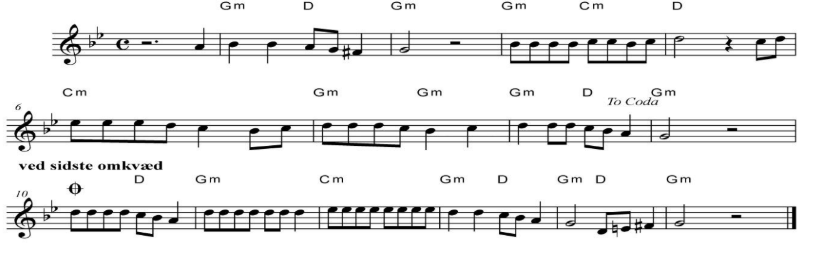
\includegraphics[width=1\textwidth]{Røvfar.png}
\end{figure*}
Mit navn det er Thorvald og jeg er kriger\\
Nu skal i høre om min færd\\
Jeg drog af sted fra min landsby Brotland\\
Ud for at vise mit sande værd\\
Min rejse var lang og fyldt med fare\\
Som ingen anden vil´ kunne klare\\
\\
Sikke noget blær, sikke noget blær\\
Dyp ham i tjære og rul ham i fjer\\
Sikke noget blær, sikke noget blær\\
Dyp ham i tjære og rul ham i fjer\\
\\
Jeg drog mod nord på min mægtige ganger\\
Og kom snart til kæmpernes store slot\\
Der smadre jeg porten og banked´ dem alle\\
Og blev derfor udnævnt til kæmpernes drot\\
Men konge jobbet var ikke mig\\
Så jeg fanged´ en bjørn og red min vej\\
\\
Sikke noget blær…\\
\\
Jeg drog mod syd for at finde solen\\
Og travede hen over ørknens sand\\
Hvad så jeg der komme i det fjerne\\
En hær af vampyrer, mindst 1000 mand\\
Godt jeg havde et stort hvidløg\\
og vampyrerne gik alle op i røg\\
\\
Sikke noget blær…\\
\\
Min bjørn den døde der i syden\\
Så vest over gik jeg nu til fods\\
Der blev jeg fanget af 700 trolde\\
der alle ville banke mig til blods\\
Men så meget som en skræmme fik jeg ikke\\
For jeg sparkede dem i deres store pi..!\\
MAVER!\\
\\
Sikke noget blær…\\
\\
Så tog jeg til havet og svømmede over\\
Langt mod øst lå en kæmpe strand\\
Der så jeg en krabbe på 10.000 kg\\
Liggende der imellem mig og land\\
Men krabben den blev nu aldrig min død\\
Og til middag der spiste jeg krabbens kød\\
\\
Sikke noget blær…\\
\\
I nord, i syd, i øst og vesten\\
Der regnes jeg for en mægtig mand\\
Min titel vil nu og for altid være:\\
Den største kriger i dette land\\
Og skulle min sang være løgn og blær\\
Så dyp mig i tjære og rul mig i fjer\\
\\
Sikke noget blær…\\
Sikke noget blær…

\subsection*{Reklamer}

\subsubsection*{Bliv rig uden at arbejde!}

Handelskompagniet giver dig en \textbf{eksklusiv mulighed} for at blive rig uden at løfte en finger! \\[0.5em]

Tjen op til \textbf{500 Fjend per dag}! \\[0.5em]

Alt du skal gøre, er at samle \textbf{Kongetand}! Handelskompagniet opkøber i øjeblikket alle de kongetand, vi kan få fat i. \\[0.5em]

Når du har bevist, at du kan samle 3 kongetand, får du \textbf{eksklusive rettigheder} til at oprette dit eget indsamlingskompagni! \\[1em]

\textit{Sådan fungerer det:}
\begin{itemize}
  \item Du samler 3 kongetander.
  \item Du finder 3 venner, der arbejder under dig.
  \item Hver af dem samler 3 kongetand til dig. Du har nu 9!
  \item Når de finder 3 venner hver, får du hele 36 kongetand!
\end{itemize}

Med vores atraktive handelsrate tilbyder vi \textbf{5 HKG}\footnote{Handelskompagni Guld} per kongetand. \\[0.5em]

Beviser du dit værd, bliver du udpeget til at være den officielle \textit{"Viceformand for eksklusiv kongetandsdistribution og indsamling"}.\footnote{Bevis for denne titel koster 5000 HKG eller 50 Fjend.} \\[1em]

\textbf{Kontakt din lokale repræsentant for Handelskompagniet i dag!}

\separator

% ====== Back matter (optional) ======
\section*{Kontakt}
Redaktionen, 1864 Salezstad

Ønsker du en artikel i Den Rullende Sten er det altid muligt at betale 15 Fjend for en 1 sides artikel.

\end{document}
